\section{PIR}

{分一下单服务器和多服务器}

我们首先给出一个PIR的具体定义。

\begin{definition}[PIR]
    一个\textit{PIR}方案$\Pi$允许客户端从数据库$\db$中检索记录$\db_\dbidx$,而不向$\servercount$个服务器中任何一个泄露索引$\dbidx$。该方案由算法元组$\Pi = (Setup, Query, Answer, Reconstruct)$组成:
    \begin{itemize}[leftmargin=*]
        \item $Setup(1^\lambda,\dbsize) \rightarrow ck$。给定数据库大小$\dbsize$和安全参数$\lambda$,生成公共参数$ck$。
        \item $Query(ck, \dbidx) \rightarrow \query$。给定公共参数$ck$和要查询的索引$\dbidx$,生成查询$\query$。
        \item $Answer(\db, \query) \rightarrow \answer$。给定查询$\query$,生成回答$\answer$。
        \item $Reconstruct(\answer) \rightarrow \db_\dbidx$。给定回答$\answer$,重构出记录$\db_\dbidx$。
    \end{itemize}
    在这一算法中,我们假设$\servercount$个服务器不能共谋。该方案需要满足两个基本性质:\textbf{正确性}和\textbf{隐私性}。
    \begin{itemize}[leftmargin=*]
        \item \textbf{正确性}:对于任意安全参数$\lambda$,对于任意数据库$\db$和索引$\dbidx$,对于任意多项式次数的查询索引序列$\{\dbidx_0,\dbidx_1, \dots\}$。如果$\servercount$个服务器和客户端按照$\Pi$诚实执行,客户端以概率$1-\negl(\lambda)$输出$\{\db_{\dbidx_0},\db_{\dbidx_1}, \dots\}$。
        \item \textbf{隐私性}:对于任意安全参数$\lambda$,对于任意数据库$\db$,对于任意多项式次数的查询索引序列$\{\dbidx_0,\dbidx_1, \dots\}$。如果$\servercount$个服务器和客户端按照$\Pi$诚实执行,$\servercount$个服务器区分$\dbidx$与一随机索引$\dbidx'$的概率小于$\negl(\lambda)$。
    \end{itemize}
    对于正确性和隐私性更形式化的定义将在后文中给出。
\end{definition}

\paragraph{线性复杂度的PIR}
如相关工作中所述,PIR的性质限制了单次查询的效率。Beimel\cite{C:BeiIshMal00}等人证明了,服务器在单次查询中,运行时间至少是线性的。这意味着,对于一个大小为$\dbsize$的数据库,服务器至少需要$O(\dbsize)$的时间来处理一个查询。这一结论是PIR的一个基本性质,也是PIR的一个重要局限。即便目前有许多工作能够将这一复杂度中的常数项降到一个较小的值,但是仍不能改变线性复杂度的基本事实。一旦数据库规模拓展,PIR的效率就会受到严重影响。本文的研究不涉及线性复杂度的PIR,因此不再详细讨论。

\subsection{亚线性复杂度的PIR}
尽管PIR的性质限制了单次查询的效率,但是我们仍然可以将多次PIR的均摊复杂度降到亚线性。需要注意的是,亚线性复杂度的PIR包含了两个阶段:\textit{离线预处理阶段}和\textit{在线查询阶段}。在预处理阶段,客户端与服务器并不进行真正的请求,仅仅生成一些用于加速查询的辅助信息,这些信息被称为 $Hint$。在查询阶段,客户端使用 $Hint$ 来加速查询。离线预处理的复杂度往往仍是线性的,而进行在线查询的复杂度则是亚线性的。将预处理的复杂度均摊到一定数量的查询中,我们可以得到亚线性复杂度的PIR。在此我们给出一个典型的离线-在线PIR定义。

\begin{definition}[离线-在线PIR]
    一个\textit{离线-在线PIR}方案$\Pi$允许客户端从数据库$\db$中检索记录$\db_\dbidx$,而不向$\servercount$个服务器中任何一个泄露索引$\dbidx$。该方案由算法元组$\Pi = (Setup, Hint, Query, Answer, Reconstruct, Refresh)$组成:
    离线部分:
    \begin{itemize}[leftmargin=*]
        \item $Setup(1^\lambda,\dbsize) \rightarrow \query_\hint$。给定数据库大小$\dbsize$和安全参数$\lambda$,生成$Hint$查询$\query_\hint$。
        \item $Hint(\db, \query_\hint) \rightarrow \hint$。给定数据库$\db$和$Hint$查询$\query_\hint$,生成$Hint$ $\hint$。
    \end{itemize}
    在线部分:
    \begin{itemize}[leftmargin=*]
        \item $Query(\hint, \dbidx) \rightarrow (\query, \clientstate)$。给定$Hint$ $\hint$和要查询的索引$\dbidx$,生成查询$\query$。注意,查询$\query$可能包含多个子查询。客户端生成并保存一个私有状态$\clientstate$。
        \item $Answer(\db, \query) \rightarrow \answer$。给定查询$\query$,生成回答$\answer$。
        \item $Reconstruct(\clientstate, \hint, \answer) \rightarrow \db_\dbidx$。给定回答$\answer$,使用$Hint$ $\hint$和私有状态$\clientstate$重构出记录$\db_\dbidx$。
        \item $Refresh(\clientstate, \hint, \answer) \rightarrow \hint$。给定回答$\answer$和私有状态$\clientstate$,更新$Hint$ $\hint$。
    \end{itemize}
    在这一算法中,我们仍假设$\servercount$个服务器不能共谋。该方案需要满足相同的两个基本性质:\textbf{正确性}和\textbf{隐私性}。其定义与PIR的定义类似,这里不再赘述。
\end{definition}

\begin{figure}
    \centering
    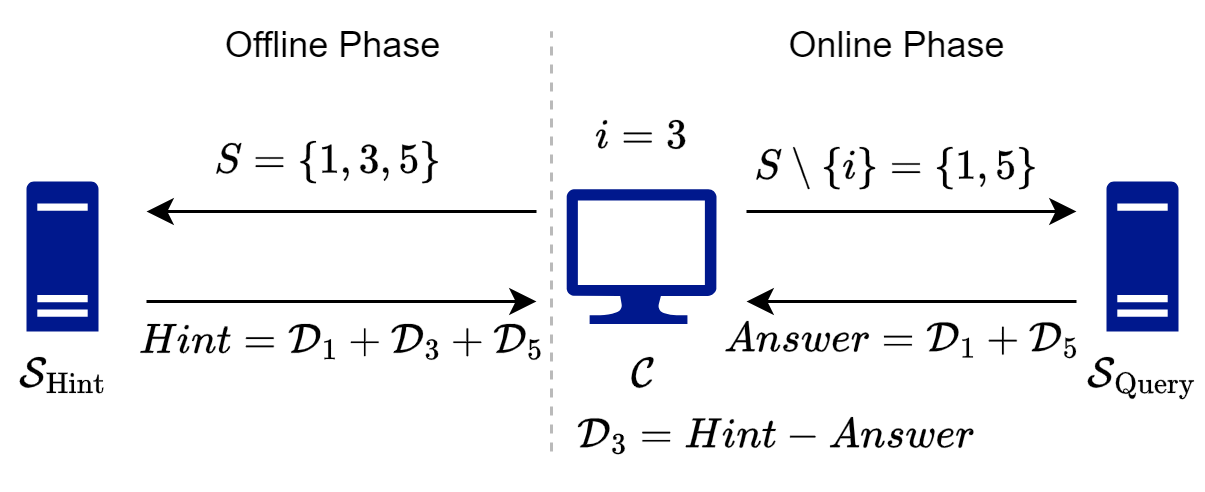
\includegraphics[width=0.5\textwidth]{figure/ck20.png}
    \caption{CK20~\cite{EC:CorKog20} 协议的一个例子。}
    \label{fig:CK20}
\end{figure}

在这些协议中,$Hint$通常由一个包含数据库$\db$中某些索引的集合,以及从这些索引对应的记录中计算出的校验值组成。本文使用Hint这个词时,除非特别指明,否则均为兼指集合与校验值。